\scanpage{46}
\margin{-- 176 --}
\margin{IX}
un homomorphisme canonique
\[
(13.4.2)\qquad\mathcal E=\uline{R}\otimes_{\mathbb Z}\uline{O}_S\longrightarrow\uline{E},
\]
dont le noyau sera noté $\uline{F}(A)$ ou simplement $\uline{F}$, de sorte qu'on a une suite exacte

(13.4.3)\quad\diagram{\begin{tikzcd}
0\arrow[r]&\uline{F}\arrow[r]&\mathcal E\arrow[r]&\uline{E}
\end{tikzcd}}.

Le cas le plus intéressant est celui où l'homomorphisme (13.4.2) est un épimorphisme, i.e. où pour tout $s\in S$, $R_s$ engendre le vectoriel complexe $E_s$. Dans ce cas on trouve donc une suite exacte

(13.4.4)\quad\diagram{\begin{tikzcd}
0\arrow[r]&\uline{F}\arrow[r]&\mathcal E\arrow[r]&\uline{E}\arrow[r]&0
\end{tikzcd}},

et si $R$ est localement constant, c'est là une suite exacte courte de Modules localement libres sur $S$. La connaissance du couple $(E,R)$ est alors équivalente à celle du couple $(R,\uline{F})$, où $R$ est un groupe analytique localement constant sur $S$ à fibres des $\mathbb Z$-Modules libres de type fini, et $\uline{F}$ est un sous-Module localement facteur direct de $\mathcal E=\uline{R}\otimes_{\mathbb Z}\uline{O}_S$, tel que l'on ait de plus la relation
\[
(13.4.5)\qquad\uline{F}\cap\uline{R}=0.
\]
Du point de vue des structures de Hodge, il y a lieu de regarder $\mathcal E$ comme filtré par la ``\uline{filtration de Hodge}''
\[
(13.4.6)\qquad\operatorname{Fil}^1(\mathcal E)=\mathcal E,\quad\operatorname{Fil}^0(\mathcal E)=\uline{F},\quad\operatorname{Fil}^{-1}(\mathcal E)=0.
\]
Notons que la suite exacte (13.4.3) dépend encore fonctoriellement du groupe analytique $A$ sur $S$, et qu'elle commute aux changements de base quelconques.
\figure{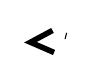
\begin{tikzpicture}\draw[line width=2pt] (.28,.15)--(0,0)--(.3,-.13);\draw (.46,.12)--(.44,.04);\end{tikzpicture}}
\margin{494}
\fbox{494}
\mspage{45}
